\section{Continuous-Time System Modeling}

%%%%%%%%%%%%%%%%%%%%%%%%%%%%%%%%%%%%%%%%%%%%%%%%%%%%%%%%%%%%%%%%%%%
\subsection{Dynamical Systems with Inputs and Outputs}
\label{sec:theory_dynamical_systems}
A model is a mathematical representation of a real system.
It is used to describe the system behavior and to answer questions by analysis or simulation.
The same physical system can be represented by different models.
The choice of model depends on the question of interest and on the required level of detail \cite{astrom_feedback_2008, karnopp_system_2012}.

A dynamical system is a system whose behavior changes over time.
In such systems, the effect of an action does not occur instantaneously.
Instead, the future behavior depends on the current condition of the system and on external influences.
Examples are mechanical motion, electrical circuits, and thermal processes \cite{astrom_feedback_2008}.

In engineering, complex systems are usually described as compositions of smaller subsystems or components.
Each component interacts with its environment through inputs and outputs.
Inputs represent external influences acting on the component.
Outputs represent variables that are provided to other components or to the environment.
This input-output view is useful because it supports the modular description of larger systems from connected subsystems \cite{karnopp_system_2012}.

In addition to inputs and outputs, a dynamical system is characterized by its state.
The state is a set of variables that contains the information required to predict the future evolution of the system for a given input.
The set of all possible states is called the state space.
For physical systems, state variables often represent quantities such as position, velocity, momentum, or stored energy \cite{astrom_feedback_2008,karnopp_system_2012}.

A common representation of continuous-time dynamical systems is the state-space form
\begin{equation}
    \dot{x} = f(x,u,t), \qquad y = h(x,u,t),
\end{equation}
where $x$ is the state vector, $u$ is the input vector, and $y$ is the output vector.
The function $f$ describes the time evolution of the state.
The function $h$ defines how the outputs are obtained from the state and the inputs.
If the functions do not depend explicitly on time, the system is called time-invariant \cite{astrom_feedback_2008}.

As a running example used throughout this chapter, we consider a rigid pendulum of
rod length $L$, mass $m$, and moment of inertia $I$, driven by a torque
$\tau$ at the hinge (Figure~\ref{fig:pendulum_simple}).

\begin{figure}[htbp]
    \centering
    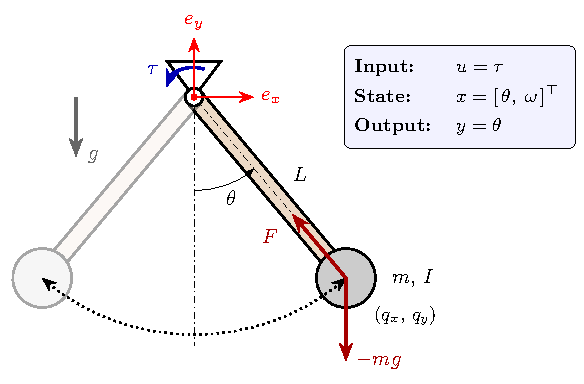
\includegraphics[width=0.75\textwidth]{figures/2_theoretical_background/pendulum_simple.pdf}
    \caption{Simple pendulum with torque input $\tau$, angle $\theta$, rod length $L$,
             mass $m$, and moment of inertia $I$.
             The system serves as a running example throughout
             Chapter~\ref{chap:foundations}.}
    \label{fig:pendulum_simple}
\end{figure}

The angular position $\theta$ and angular velocity $\omega = \dot{\theta}$ are the natural state variables since they contain exactly the information required to predict the future motion for any given input torque.
The equation of motion is $I\ddot{\theta} = \tau - mgL\sin\theta$.
With $x = [\theta,\,\omega]^\top$, $u = \tau$, and $y = \theta$ gives the state-space form

\begin{equation}
    \dot{x}_1 = x_2,
    \qquad
    \dot{x}_2 = \frac{1}{I}\bigl(u - mgL\sin(x_1)\bigr),
    \qquad
    y = x_1.
    \label{eq:pendulum_ode}
\end{equation}
The output $\theta$ depends only on the state $x_1$ and not directly on the current
input $\tau$, so the system has no direct feedthrough.
The structural property of direct feedthrough is developed further in
Section~\ref{sec:theory_direct_feedthrough}.

%%%%%%%%%%%%%%%%%%%%%%%%%%%%%%%%%%%%%%%%%%%%%%%%%%%%%%%%%%%%%%%%%%%
\subsection{Ordinary and Differential-Algebraic Equations}
\label{sec:theory_ode_dae}

Many continuous-time systems can be described by ordinary differential equations.
In this case, the time derivative of the state is given explicitly as a function of the current state, the input, and time \cite{kunkel_differential-algebraic_2024,css_cellier_kofman}.
A general nonlinear ODE can be written as
\begin{equation}
    \dot{x} = f(x,u,t),
\end{equation}
where $x$ is the state vector and $u$ is the input vector.

However, not all continuous-time models are naturally expressed in explicit ODE form.
In many physical systems, algebraic constraints are present in addition to the differential equations.
These constraints may arise, for example, from geometric relations, constitutive relations, or conservation laws \cite{css_cellier_kofman, karnopp_system_2012}.
Such models are more naturally written as differential-algebraic equations.

A general DAE can be written in implicit form as
\begin{equation}
    G(t,z,\dot{z},u) = 0,
\end{equation}
where $z$ contains the model variables and $u$ denotes the input.
In contrast to an ODE, the derivatives are not given explicitly.
Instead, differential and algebraic relations are stated together \cite{kunkel_differential-algebraic_2024}.

A common semi-explicit form of a DAE is
\begin{align}
    \dot{x} &= f(x,w,u,t), \\
    0 &= g(x,w,u,t),
\end{align}
where $x$ contains the differential states and $w$ contains algebraic variables.
The first equation describes the time evolution of the states, while the second equation imposes algebraic constraints that must hold at every time instant.
This representation is useful because it separates dynamic behavior from purely algebraic relations \cite{kunkel_differential-algebraic_2024,css_cellier_kofman}.

In contrast to ODEs, a DAE does not in general admit arbitrary initial values.
The initial state must be consistent with the algebraic constraints.
In addition, DAEs are often classified by an index that reflects the structural difficulty of the problem.
Higher-index systems are generally harder to analyse and simulate \cite{kunkel_differential-algebraic_2024}.

The pendulum introduced in Section~\ref{sec:theory_dynamical_systems} provides a simple example.
In generalized coordinates, its dynamics are described by the ODE~\eqref{eq:pendulum_ode}.
The same physical system can also be formulated in Cartesian coordinates $(q_x,\,q_y)$ for the bob position, related to the polar angle by $q_x = L\sin\theta$ and $q_y = -L\cos\theta$.
In this representation, the rigid rod introduces the geometric constraint that the bob must remain on a circle of radius $L$.

Applying Newton's second law in the Cartesian directions and enforcing the rod rigidity yields \cite{Modelica_Fritzson}
\begin{align}
    m\dot{v}_x &= -\frac{q_x}{L}\,F,              \label{eq:pendulum_dae_x}\\
    m\dot{v}_y &= -\frac{q_y}{L}\,F - mg,         \label{eq:pendulum_dae_y}\\
    \dot{q}_x  &= v_x,                            \label{eq:pendulum_dae_vx}\\
    \dot{q}_y  &= v_y,                            \label{eq:pendulum_dae_vy}\\
    0          &= q_x^2 + q_y^2 - L^2.           \label{eq:pendulum_constraint}
\end{align}
Here, $(q_x,q_y,v_x,v_y)$ are the position and velocity components and $F$ is the scalar constraint force in the rod.
Equations~\eqref{eq:pendulum_dae_x}--\eqref{eq:pendulum_dae_vy} are differential equations, whereas \eqref{eq:pendulum_constraint} is an algebraic constraint.
In the semi-explicit form introduced above, $(q_x,q_y,v_x,v_y)$ are the differential variables and $F$ is the algebraic variable.

This formulation shows that the same physical system may appear either as an ODE or as a DAE, depending on the choice of variables and coordinates.
The ODE form in generalized coordinates eliminates the geometric constraint explicitly.
The Cartesian formulation retains the constraint and therefore leads naturally to a DAE.
This distinction is important in physical modeling, where algebraic constraints often arise directly from the chosen representation.

In addition to such internal constraints, algebraic relations may also arise when subsystems are connected through their interfaces.
These connection-induced algebraic loops are introduced in the following subsection.

%%%%%%%%%%%%%%%%%%%%%%%%%%%%%%%%%%%%%%%%%%%%%%%%%%%%%%%%%%%%%%%%%%%
\subsection{Direct Feedthrough and Interface Variables}
\label{sec:theory_direct_feedthrough}

Building on the input-output view introduced in Section~\ref{sec:theory_dynamical_systems}, consider a subsystem represented by
\begin{equation}
    \dot{x} = f(x,u,t),
    \qquad
    y = h(x,u,t),
\end{equation}
where $x$ is the state vector, $u$ is the input vector, and $y$ is the output vector.
A subsystem has \emph{direct feedthrough} if the current output depends directly on the current input.
If the output depends only on the state, then no direct feedthrough is present.

In the linear time-invariant case,
\begin{equation}
    \dot{x} = Ax + Bu,
    \qquad
    y = Cx + Du,
\end{equation}
direct feedthrough is present if the matrix $D$ is nonzero \cite{astrom_feedback_2008}.
More generally, direct feedthrough is a structural property of the output relation $h(x,u,t)$.

This distinction becomes important when subsystems are connected through their interfaces.
If a subsystem output depends instantaneously on its input, then a connection introduces an immediate dependency between the connected variables.
If such dependencies form a closed loop, the coupled system can no longer be evaluated by a simple sequential propagation of signals.
Instead, the interface variables must satisfy a set of algebraic equations simultaneously.

A simple example is obtained by two interconnected subsystems
\begin{align}
    \dot{x}_A &= f_A(x_A,u_A,t),
    & y_A &= h_A(x_A,u_A,t), \\
    \dot{x}_B &= f_B(x_B,u_B,t),
    & y_B &= h_B(x_B,u_B,t),
\end{align}
with the interconnection conditions
\begin{equation}
    u_A = y_B,
    \qquad
    u_B = y_A.
\end{equation}
If both $y_A$ and $y_B$ depend directly on the current inputs $u_A$ and $u_B$, then the coupled interface variables must be determined simultaneously.
The interconnection therefore introduces an algebraic loop.

If, in contrast, at least one subsystem output depends only on its internal state, the instantaneous circular dependency is broken and the coupled system may be evaluated sequentially.
Direct feedthrough is therefore an important structural property in interconnected continuous-time models.
It determines whether interface equations merely transmit already available values or whether they introduce additional algebraic constraints across subsystem boundaries.

Such interface-induced algebraic relations are conceptually distinct from the internal algebraic constraints discussed in Section~\ref{sec:theory_ode_dae}.
The Cartesian pendulum example contains an internal geometric constraint within a single model.
By contrast, direct feedthrough concerns algebraic dependencies that arise from the interconnection of subsystems through their inputs and outputs.

These structural properties, direct feedthrough and the resulting algebraic loops, are used in later sections to derive component execution order and to detect and resolve algebraic dependencies in coupled co-simulation systems.